\documentclass[10pt,twocolumn,letterpaper]{article}

\usepackage{cvpr}
\usepackage{times}
\usepackage{epsfig}
\usepackage{graphicx}
\usepackage{amsmath}
\usepackage{caption}
\usepackage{subcaption}
\usepackage{booktabs}
\usepackage{amssymb}
%\usepackage{hyperref}

% Include other packages here, before hyperref.

% If you comment hyperref and then uncomment it, you should delete
% egpaper.aux before re-running latex.  (Or just hit 'q' on the first latex
% run, let it finish, and you should be clear).
\usepackage[breaklinks=true,bookmarks=false]{hyperref}

\cvprfinalcopy % *** Uncomment this line for the final submission

\def\cvprPaperID{****} % *** Enter the CVPR Paper ID here
\def\httilde{\mbox{\tt\raisebox{-.5ex}{\symbol{126}}}}

% Pages are numbered in submission mode, and unnumbered in camera-ready
%\ifcvprfinal\pagestyle{empty}\fi
%\setcounter{page}{4321}
\begin{document}

%%%%%%%%% TITLE
\title{Assignment 1: Support Vector Machines}

\author{Moaz Mohamed\\
The University of Adelaide\\
Adelaide SA 5005\\
{\tt\small a1779177@student.adelaide.edu.au}
% For a paper whose authors are all at the same institution,
% omit the following lines up until the closing ``}''.
% Additional authors and addresses can be added with ``\and'',
% just like the second author.
% To save space, use either the email address or home page, not both

}

\maketitle
%\thispagestyle{empty}

%%%%%%%%% ABSTRACT
%\begin{abstract}
  % The ABSTRACT is to be in fully-justified italicized text, at the top
  % of the left-hand column, below the author and affiliation
  % information. Use the word ``Abstract'' as the title, in 12-point
  % Times, boldface type, centered relative to the column, initially
  % capitalized. The abstract is to be in 10-point, single-spaced type.
  % Leave two blank lines after the Abstract, then begin the main text.
 %  Look at previous CVPR abstracts to get a feel for style and length.
%\end{abstract}

%%%%%%%%% BODY TEXT
\section{Introduction}

Over the last few years, Machine learning had a significant impact in the current technological landscape. 
The application of numerous Deep learning algorithms have been implemented in different sectors. In this paper Support vector machine (SVM) algorithm will be explored and its performance will be investigated on classification task on the provided dataset.In addition to a complete review of the SVM algorithm describing its strength and weakness.
%-------------------------------------------------------------------------
\section{Methodology and Background}



\subsection{Support Vector Machines}

A famous approach to pattern recognition is using Support Vector Machines (SVM). Which in hindsight is very similar to the perceptron algorithm but SVM ensures finding a hyperplane  that can separate between the two classes with maximum margin. the decision for either positive or negative classification follows the eq \ref{eq:dbsvm}. 


\begin{equation}
y_{i}\left(w x_{i}+b\right) \geq 1
\label{eq:dbsvm}
\end{equation}

for the data points that lie exactly on the support vector boundary. 
\begin{equation}
y_{i}\left(w x_{i}+b\right)-1=0
\label{eq:svm-1}
\end{equation}

finding the width for the maximum margin will depend on finding the distance between the negative and positive points that exist on the boundary $\left(x_{p}-x_{n}\right)$ multiplying by $\frac{\bar{w}}{\|w\|}$ as unit vector provides the width. 

\begin{equation}
\left(x_{p}-x_{n}\right) \times \frac{\bar{w}}{\|w\|}
\end{equation}

using eq \ref{eq:svm-1} the term that need to be maximized comes naturally as $\frac{2}{\|w\|}$ or for minimization as $\frac{1}{2} \times\|w\|^{2}$

\begin{equation}
\begin{array}{l}
\frac{1}{\|w\|} \times\left(x_{p} w-x_{n} w\right) \\
\frac{1}{\|w\|} \times([1-b]+[1+b])
\end{array}
\end{equation}


\begin{equation}
\begin{array}{l}
\frac{2}{\|w\|} \\ \\
\frac{1}{2} \times\|w\|^{2}
\end{array}
\end{equation}


thus the margin is 

\begin{equation}
\frac{1}{2} \times\|w\|^{2}
\end{equation}


which can be constructed as a function to 

minimize 
\begin{equation}
j\left( w\right) =\dfrac{1}{2}\times \left\| w\right\| ^{2}
\end{equation}

subject to 
\begin{equation}
y_{i}\left( w^{T}x_{i}+b\right) \geq 1 , \forall j
\end{equation}

Such formulation does work on finding the optimal hyperplane and it can be solved with  optimization tool such as CVXOPT or MOSER. a slack variable can also be added to relax the SVM with $C$ as regularization parameter. 

minimization of 

\begin{equation}
\frac{1}{2} \times\|w\|^{2}+c\times \dfrac{1}{n}\sum ^{n}_{i=1}\xi _{i}
\end{equation}

subject to 

\begin{equation}
\begin{aligned}y_{i}\left( w^{T}x_{i}+b\right) \geq 1-\xi i\\
\xi _{i}\geq 0,\forall n\end{aligned}
\end{equation}


Kuhn-Tucker theorem and Lagrange multipliers can be utilized to drive the previous problem from primal problem to dual problem. 

\begin{equation}
L_{D}\left( \alpha \right) =\sum ^{n}_{i}\alpha _{i}-\dfrac{1}{2}\sum ^{n}_{i=1}\sum ^{n}_{j=1}\alpha _{i}\alpha _{j}y_{i}y_{j} <X_{i}^{T}X_{j} >
\label{eqn:l}
\end{equation}

subject to for (non-separable case)
\begin{equation}
0 \leq \alpha_{i} \leq C/n , \forall i,\sum ^{n}_{i=1}\alpha _{i}y_{i}=0
\end{equation}

or subject to for (separable case)

\begin{equation}
\alpha_{i} \geq 0 , \forall i,\sum ^{n}_{i=1}\alpha _{i}y_{i}=0
\end{equation}

and the $\overrightarrow{w}$ and the bias term can be calculated as follows. 
\begin{equation}
w=\sum ^{n}_{i=1}\alpha _{i}y_{j}x_{i}
\label{eqn:weight}
\end{equation}

\begin{equation}
b =\dfrac{1}{y_{j}}-w^{T}x_{j}
\end{equation}
 
It is interesting to note that in equation \ref{eqn:weight} the weight vector can be formulated as summation of alpha, label and the support vectors. Hence the number of the support vectors is depended on $\alpha _{i}$ as some values of $\alpha _{i}$ will be zero.
instead of in the primal problem where the $\overrightarrow{w}$ is obtained directly from solving the primal optimization problem which can be computationally expensive as the number of dimensions increases hence in the primal problem all the points have to be queried unlike in Dual problem $\overrightarrow{w}$ can be obtained from only non zero values of $\alpha _{i}$. Also such difference allows for the usage for something called the "Kernel Trick".
 
\begin{equation}
L_{D}\left( \alpha \right) =\sum ^{n}_{i=1}\alpha _{i}-\dfrac{1}{2}\sum ^{n}_{i=1}\sum ^{n}_{j=1}\alpha _{i}\alpha _{j}y_{i}y_{j}K\left( x_{j},x_{i}\right) 
\label{eqn:lk}
\end{equation} 


\begin{figure}[h!]
  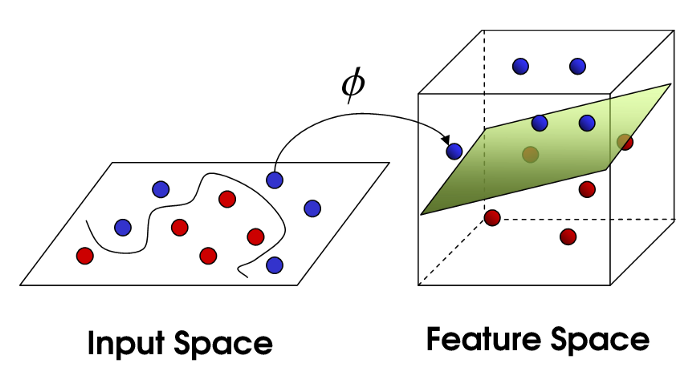
\includegraphics[width=\linewidth]{kernel.png}
  \caption{Mapping}
  \label{fig:kernel}
\end{figure}


\begin{equation}
K\left( x_{j},x_{i}\right) =\left( x_{i}^{T}x_{j}+1\right) ^{p}
\label{eq:polyk}
\end{equation}


\begin{equation}
K\left( x_{i},x_{j}\right) =\exp \left( -\dfrac{1}{2\sigma ^{2}}\times \left\| x_{j}-x_{i}\right\| ^{2}\right) 
\label{eq:rbfk}
\end{equation}

The optimization problems for both equations \ref{eqn:lk} and \ref{eqn:l} except for the $( x_{j},x_{i})$ in equation \ref{eqn:lk} is being applied to a kernel (Ex eq \ref{eq:polyk} and \ref{eq:rbfk}) and the data is being projected into higher dimensions. here the SVM is exploiting cover's theorem."A complex pattern-classification problem, cast in a high-dimensional space non-linearly, is more likely to be linearly separable than in a low-dimensional space, provided that the space is not densely populated." \cite{Cover1965} Which increases the complexity of the SVM by applying the kernel and enabling it to classify classes even in non-separable cases as demonstrated in figure \ref{fig:kernel} and \ref{fig:svm_exp_k}

\section{Experimental Analysis.}

\subsection{SVM Primal and Dual}
Sklearn toy datasets (classification and circles) have been used to for demonstration purposes. By utilizing the support vectors in eq \ref{eqn:weight} SVM is able to find the support vectors that can maximize the margin between the two classes as demonstrated in equation \ref{eqn:l} but SVM without utilizing a kernel SVM has the same weakness as Perceptron \cite{Rosenblatt1958} \cite{Minsky1969} \cite{Murphy2017} in that regard. But when a kernel is utilized project the data into higher dimensions SVM is capable of finding a hyperplane between the two classes as demonstrated in figure \ref{fig:svm_exp_k}.

\begin{figure}[htb]
  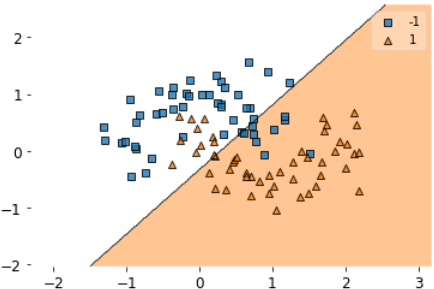
\includegraphics[width=\linewidth]{svm_lin_non_sep.png}
  \caption{SVM decision boundary in non-linearly separable data}
  \label{fig:svm_exp_non_lin}
\end{figure}

\vspace{3.00mm} 

\begin{figure}[htb]
  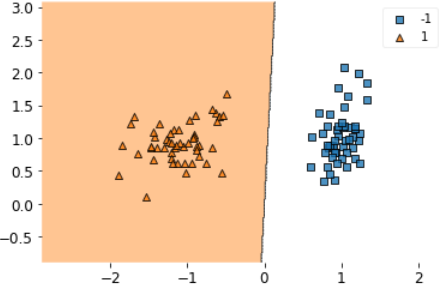
\includegraphics[width=\linewidth]{svm_lin_sep.png}
  \caption{SVM decision boundary in linearly separable data}
  \label{fig:svm_exp_lin}
\end{figure}

\vspace{50.00mm} 

\begin{figure}[htb]
  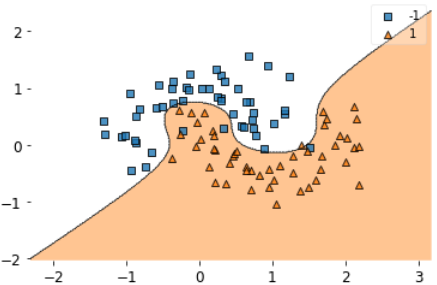
\includegraphics[width=\linewidth]{svm_k_non.png}
  \caption{SVM with polynomial kernel applied. Decision boundary in non-linearly separable data}
  \label{fig:svm_exp_k}
\end{figure}





\subsection{Performance on toy and provided data-set}
In table \ref{tab:SVM_soft} and \ref{tab:SVM_hard} are the wights and biases produced by using CVXPY package to solve both primal and dual problems and the comparison with sklearn. As it can be seen in both tables the values are quite quite similar and acceptable error margin on the sklearn toy datasets. the performance on the provided dataset is shown in \ref{tab:SVM_soft_data} with the same C parameters for all versions of SVM. with aggressive hyper-parameter tuning obtaining even a higher performance should be possible using grid-search with cross validation in mind but due to limited computation resources that have been abandoned to concentrate on the mathematical foundation of the algorithm itself.


\begin{table}[htb]
\centering
\begin{tabular}{|l|l|l|l|} 
\toprule
Algorithm   & W                           & bias       & accuracy  \\ 
\hline
Dual Soft   & {[} 0.75893, -0.651570] & 0.290155 & 59\%      \\ 
\hline
Primal Soft & {[} 0.75884, -0.651509] & 0.290233 & 59\%      \\ 
\hline
sklearn     & {[} 0.75886, -0.651530] & 0.290229 & 59\%      \\
\bottomrule
\end{tabular}
\caption{SVM implementation for Soft margin}
\label{tab:SVM_soft}
\end{table}



\begin{table}[htb]
\centering
\begin{tabular}{|l|l|l|l|} 
\toprule
Algorithm   & W                        & bias      & accuracy  \\ 
\hline
Dual Hard   & {[}-1.75455, 0.077797] & 0.00377 & 100\%     \\ 
\hline
Primal Hard & {[}-1.75451, 0.077783]  & 0.0038 & 100\%     \\ 
\hline
sklearn     & {[}-1.74054, 0.077163]  & 0.0117 & 100\%     \\
\bottomrule
\end{tabular}
\caption{SVM implementation for Hard margin}
\label{tab:SVM_hard}
\end{table}



\begin{table}[htb]
\centering
\begin{tabular}{|l|l|l|l|} 
\toprule
Algorithm   & training set & testing set & C     \\ 
\hline
Dual Soft   & 97.74\%      & 96.8\%      & 1000  \\ 
\hline
Primal Soft & 97.71\%      & 96.8\%      & 1000  \\ 
\hline
sklearn     & 97.75\%      & 96.7\%      & 1000  \\
\bottomrule
\end{tabular}
\caption{SVM implementation for Soft margin on provided dataset}
\label{tab:SVM_soft_data}
\end{table}

\section{Conclusion}
Different variations of Support vector machines algorithm have been explored and analysed. mathematical formulation of all the algorithms have been studied. decision boundaries for have been made for a careful study of the behaviour of various algorithms in different data situations. Advantageous and weakness have been identified for all the explored algorithms. SVM provides a very beautiful mathematical assay for its excellent performance especially for its ability to use different kernel to suit non-linear data. the math is elegant and provides excellent intuition for what is exactly the algorithm is doing to find the pattern in the data. 


\bibliography{egbib.bib} 
\bibliographystyle{ieeetr}

\end{document}
